\chapter{Rahmen}
Erarbeitet von: Leon Kranner und Marcel Wagner \\ \\
\noindent
In diesem Kapitel wird die Vorgehensweise für die Rahmenkonstruktion des Smart Mirrors beschrieben.

\section{Rahmen Konstruktion}
\begin{enumerate}
    \item \textbf{Planung:}
Zu Beginn der Planung haben wir die Abmessungen des Displays genau vermessen, um den benötigten Platz für die Hardwarekomponenten und das Gehäuse bestimmen zu können. Es war wichtig, genügend Raum für den Raspberry Pi, die Kamera für die Gesichtserkennung, den WLAN-Stick und eventuelle Kabelverbindungen einzuplanen.

Nachdem wir die Abmessungen des Displays und den Platzbedarf für die Hardware ermittelt hatten, konnten wir den Maßstab und die endgültige Größe des Rahmens festlegen. Unser Ziel war es, einen Rahmen zu konstruieren, der sowohl funktional als auch ästhetisch ansprechend ist.

Im nächsten Schritt besuchten wir den Baumarkt, um das passende Material für unseren Rahmen auszuwählen. Wir entschieden uns schließlich für Leimholz, da es robust und gut zu verarbeiten ist.

Ursprünglich war geplant, den Rahmen mit Schrauben zusammenzubauen. Nach weiteren Überlegungen und Tests fanden wir jedoch, dass die geschraubte Konstruktion unseren ästhetischen Ansprüchen nicht gerecht wurde. Daher entschieden wir uns, das Leimholz zu verwenden und die Teile zu verleimen. Diese Methode bot uns eine stabilere und sauberere Verbindung der Rahmenteile.
    \item \textbf{Zuschneiden des Leimholzes:}
    Zu Beginn der Konstruktion wurde das Leimholz auf die gewünschte Länge zugeschnitten. Dabei war es wichtig, präzise Maße zu verwenden, um sicherzustellen, dass alle Teile des Rahmens passgenau zueinander stehen. Für den Zuschnitt wurde eine Kreissäge verwendet, um gerade und saubere Schnitte zu erzielen.
    
    \item \textbf{Gehrungsschnitt der Kanten:}
    Um eine ästhetisch ansprechende und stabile Verbindung der Rahmenteile zu gewährleisten, wurden die Kanten des Holzes auf Gehrung geschnitten. Hierzu wurde ein Gehrungssägeblatt in einem Winkel von 45 Grad eingestellt. Dieser Schritt ist entscheidend, da die Gehrungsschnitte die Stoßkanten der Rahmenteile so ausrichten, dass sie sich nahtlos und formschlüssig verbinden lassen.
    
    \item \textbf{Verleimung der Rahmenteile:}
    Nach dem Gehrungsschnitt wurden die Kanten mit Holzleim bestrichen. Es ist wichtig, den Leim gleichmäßig aufzutragen, um eine vollständige und feste Verbindung zu gewährleisten. Die Rahmenteile wurden dann sorgfältig zusammengesetzt, wobei darauf geachtet wurde, dass die Gehrungsschnitte exakt aufeinanderpassen. \\ \\
Zur Sicherstellung einer stabilen Verbindung wurden die verleimten Rahmenteile mit Schraubzwingen fixiert. Die Schraubzwingen wurden gleichmäßig verteilt angezogen, um den Druck auf alle Teile des Rahmens zu verteilen und Verformungen zu vermeiden. Die Rahmenkonstruktion wurde dann für die empfohlene Zeitspanne in den Schraubzwingen belassen, um eine vollständige Aushärtung des Leims zu gewährleisten. In der nachfolgenden Abbildung kann dar Spiegelrahmen entnommen werden.

\begin{figure}[h]
    \centering
    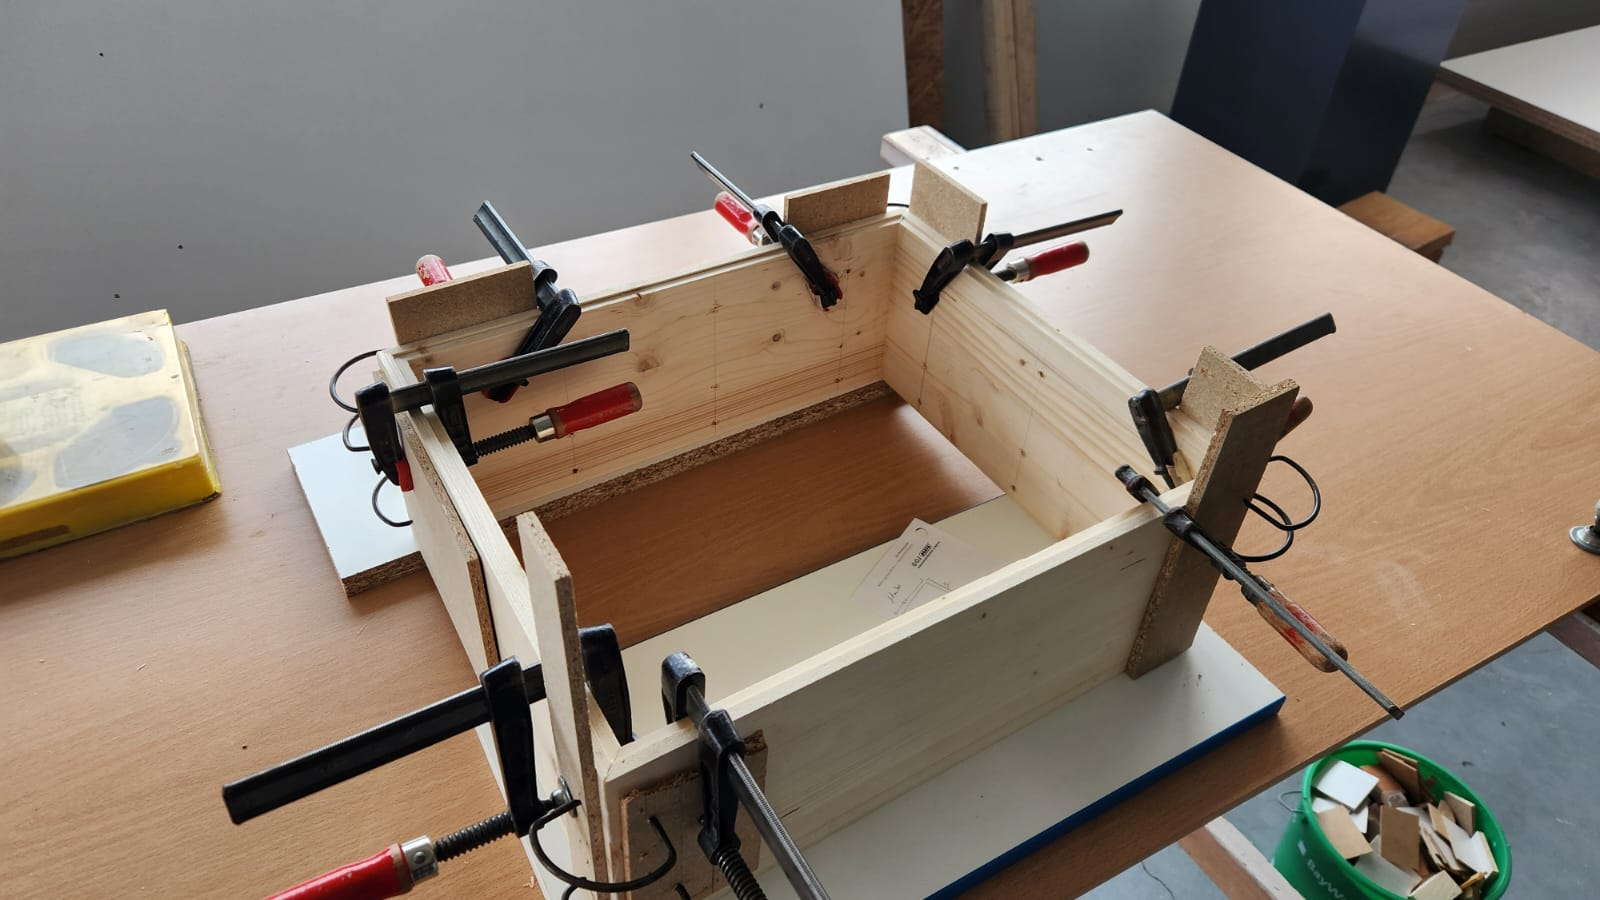
\includegraphics[width=0.5\textwidth]{pictures/Rahmen_geleimt.jpg}
  \captionsetup{justification=centering, labelformat=simple, singlelinecheck=false}
    \caption[Rahmen wurde geleimt]{Rahmen wurde geleimt\\ Quelle: eigene Darstellung}
\end{figure}
    
    \item \textbf{Befestigung der Halteleiste:}
    Nach der Aushärtung des Leims wurde eine Halteleiste angebracht. Diese Leiste dient dazu, den Spiegel sicher im Rahmen zu fixieren. Die Halteleiste wurde präzise vermessen und zugeschnitten, um optimal in den Rahmen zu passen. Sie wurde mit Holzleim und zusätzlichen Schrauben befestigt, um eine dauerhafte und sichere Fixierung zu gewährleisten.
\end{enumerate}
\begin{figure}[h]
    \centering
    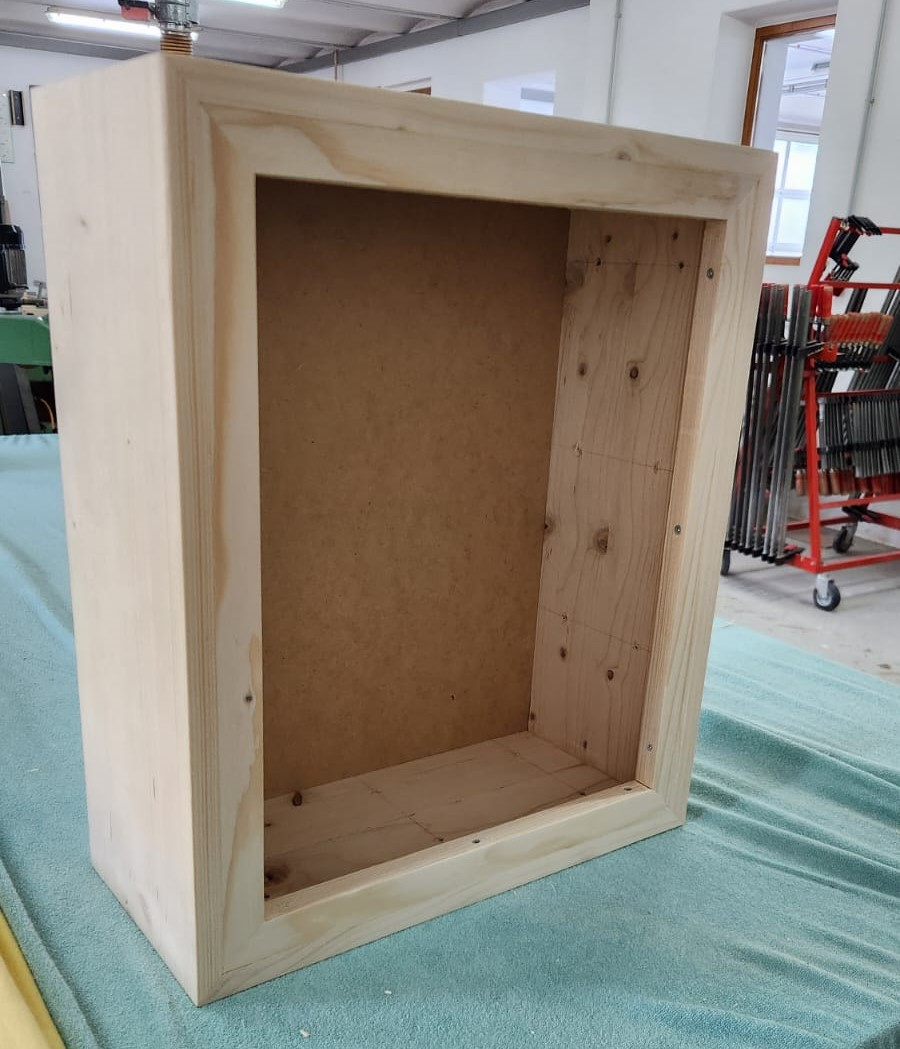
\includegraphics[width=0.3\textwidth]{pictures/Rahmen_fertig.jpg}
  \captionsetup{justification=centering, labelformat=simple, singlelinecheck=false}
    \caption[Fertiggestellter Rahmen]{Fertiggestellter Rahmen\\ Quelle: eigene Darstellung}
\end{figure}
\newpage

\section{Spiegel}
\begin{enumerate}
    \item \textbf{Auswahl des Materials:}
Ursprünglich hatten wir geplant, eine Glasscheibe für den Spiegel des Smart Mirrors zu verwenden. Da jedoch für unsere Zwecke eine Glasscheibe nicht erforderlich war und wir bereits eine Plexiglasscheibe zur Verfügung hatten, entschieden wir uns, diese zu verwenden.

    \item \textbf{Zuschnitt und Vorbereitung:}
Zunächst haben wir anhand des Rahmens abgemessen, wie groß der Spiegel sein muss, und eine Toleranz von 1 cm festgelegt. Mit Hilfe einer Stichsäge haben wir das Plexiglas auf Maß geschnitten. Anschließend haben wir die Kanten mit einer Feile entgratet und mit Schleifpapier die unebenen Stellen beseitigt.
    
    \item \textbf{Bohrungen und Befestigung:}
Um das Plexiglas später am Rahmen befestigen zu können, haben wir an den Seiten des Plexiglases Bohrungslöcher gebohrt.
    
    \item \textbf{Anbringen der Spiegelfolie:}
    Zunächst haben wir eine Spiegelglasfolie auf das Plexiglas aufgebracht. Beim Testen mit dem Bildschirm stellten wir jedoch fest, dass die Helligkeit des Displays nicht ausreichte, um den Bildschirm durch das Plexiglas und die Spiegelglasfolie zu erkennen. Aufgrund der unzureichenden Helligkeit des Displays haben wir uns für eine Sonnenschutzfolie entschieden. Diese Folie spiegelt immer noch, ermöglichte dennoch eine bessere Sicht.

\end{enumerate}
\section{Aufbau}
\begin{enumerate}
    \item \textbf{Befestigung des Plexiglases:}
Nachdem die geeignete Folie angebracht war, haben wir das Plexiglas mit Schrauben fixiert. Diese Maßnahme gewährleistete eine stabile und sichere Befestigung.

    \item \textbf{Montage des Bildschirms:}
Der erste Ansatz zur Befestigung des Bildschirms bestand darin, ein Draht von der linken zur rechten Seite des Spiegels zu spannen. Diese Lösung fixiert den Bildschirm in der gewünschten Position und verhinderte ein Verrutschen. Aufgrund der Anfälligkeit für Spielräume und der Tatsache, dass der Bildschirm nicht immer fest mit dem Plexiglas verbunden ist, entschieden wir uns jedoch, den Bildschirm mit eng anliegenden Haltern am Bilderrahmen zu fixieren. Diese Konstruktion gewährleistet eine klare und stabile Befestigung des Bildschirminhalts durch die Spiegelfolie.
    
    \item \textbf{Integration der Elektronik:}
An der Seite des Rahmens haben wir den Raspberry Pi befestigt und den Bildschirm angeschlossen. Der Raspberry Pi steuert die gesamte Funktionalität des Smart Mirrors. In der nachfolgenden Abbildung kann der befestigte Raspberry Pi an dem Spiegerrahmen entnommen werden.
\begin{figure}[h]
    \centering
    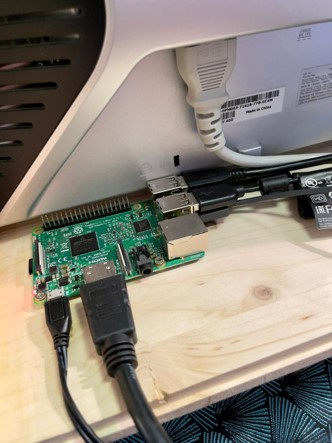
\includegraphics[width=0.3\textwidth]{pictures/Raspberry_pi_Befestigung.jpg}
  \captionsetup{justification=centering, labelformat=simple, singlelinecheck=false}
    \caption[Raspberry Pi am Rahmen befestigt]{Raspberry Pi am Rahmen befestigt\\ Quelle: eigene Darstellung}
\end{figure}
\newpage
    \item \textbf{Zusätzliche Komponenten:}
    Wir haben zudem eine Kamera für die Gesichtserkennung (Eggo AI) angeschlossen. Diese Kamera ermöglicht personalisierte Funktionen und verbessert die Benutzererfahrung. Zusätzlich haben wir einen WLAN-Stick integriert, damit die Widgets Daten aus dem Internet abrufen und mit der App kommunizieren können

\end{enumerate}

Der nachfolgende Bild zeigt den fertigen Smart Mirror.
\begin{figure}[h]
    \centering
    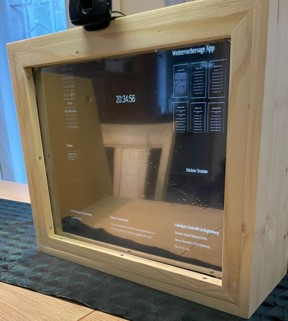
\includegraphics[width=0.3\textwidth]{pictures/Spiegel_AI.jpg}
  \captionsetup{justification=centering, labelformat=simple, singlelinecheck=false}
    \caption[Spiegel AI]{Spiegel AI\\ Quelle: eigene Darstellung}
\end{figure}